\documentclass{article}
\iffalse
This file is protected by Copyright. Please refer to the COPYRIGHT file
distributed with this source distribution.

This file is part of OpenCPI <http://www.opencpi.org>

OpenCPI is free software: you can redistribute it and/or modify it under the
terms of the GNU Lesser General Public License as published by the Free Software
Foundation, either version 3 of the License, or (at your option) any later
version.

OpenCPI is distributed in the hope that it will be useful, but WITHOUT ANY
WARRANTY; without even the implied warranty of MERCHANTABILITY or FITNESS FOR A
PARTICULAR PURPOSE. See the GNU Lesser General Public License for more details.

You should have received a copy of the GNU Lesser General Public License along
with this program. If not, see <http://www.gnu.org/licenses/>.
\fi

\author{} % Force author to be blank
%----------------------------------------------------------------------------------------
% Paper size, orientation and margins
%----------------------------------------------------------------------------------------
\usepackage{geometry}
\geometry{
	letterpaper,			% paper type
	portrait,				% text direction
	left=.75in,				% left margin
	top=.75in,				% top margin
	right=.75in,			% right margin
	bottom=.75in			% bottom margin
 }
%----------------------------------------------------------------------------------------
% Header/Footer
%----------------------------------------------------------------------------------------
\usepackage{fancyhdr} \pagestyle{fancy} % required for fancy headers
\renewcommand{\headrulewidth}{0.5pt}
\renewcommand{\footrulewidth}{0.5pt}
\rhead{\small{ANGRYVIPER Team}}
%----------------------------------------------------------------------------------------
% Appendix packages
%----------------------------------------------------------------------------------------
\usepackage[toc,page]{appendix}
%----------------------------------------------------------------------------------------
% Defined Commands & Renamed Commands
%----------------------------------------------------------------------------------------
\renewcommand{\contentsname}{Table of Contents}
\renewcommand{\listfigurename}{List of Figures}
\renewcommand{\listtablename}{List of Tables}
\newcommand{\todo}[1]{\textcolor{red}{TODO: #1}\PackageWarning{TODO:}{#1}} % To do notes
\newcommand{\code}[1]{\texttt{#1}} % For inline code snippet or command line
%----------------------------------------------------------------------------------------
% Various pacakges
%----------------------------------------------------------------------------------------
\usepackage{hyperref} % for linking urls and lists
\usepackage{graphicx} % for including pictures by file
\usepackage{listings} % for coding language styles
\usepackage{rotating} % for sideways table
\usepackage{pifont}   % for sideways table
\usepackage{pdflscape} % for landscape view
%----------------------------------------------------------------------------------------
% Table packages
%----------------------------------------------------------------------------------------
\usepackage{tabularx} % c=center,l=left,r=right,X=fill
\usepackage{float}
\floatstyle{plaintop}
\usepackage[tableposition=top]{caption}
\newcolumntype{P}[1]{>{\centering\arraybackslash}p{#1}}
\newcolumntype{M}[1]{>{\centering\arraybackslash}m{#1}}
%----------------------------------------------------------------------------------------
% Block Diagram / FSM Drawings
%----------------------------------------------------------------------------------------
\usepackage{tikz}
\usetikzlibrary{shapes,arrows,fit,positioning}
\usetikzlibrary{automata} % used for the fsm
%----------------------------------------------------------------------------------------
% Colors Used
%----------------------------------------------------------------------------------------
\usepackage{colortbl}
\definecolor{blue}{rgb}{.7,.8,.9}
\definecolor{ceruleanblue}{rgb}{0.16, 0.32, 0.75}
\definecolor{drkgreen}{rgb}{0,0.6,0}
\definecolor{deepmagenta}{rgb}{0.8, 0.0, 0.8}
\definecolor{cyan}{rgb}{0.0,0.6,0.6}
\definecolor{maroon}{rgb}{0.5,0,0}
%----------------------------------------------------------------------------------------
% Update the docTitle and docVersion per document
%----------------------------------------------------------------------------------------
\def\docTitle{Component Data Sheet}
\def\docVersion{1.2}
%----------------------------------------------------------------------------------------
\date{Version \docVersion} % Force date to be blank and override date with version
\title{\docTitle}
\lhead{\small{\docTitle}}

\def\comp{matchstiq\_z1\_tx}
\def\Comp{Matchstiq-Z1 TX}
\graphicspath{ {figures/} }

\begin{document}

\section*{Summary - \Comp}
\begin{tabular}{|c|M{13.5cm}|}
	\hline
	\rowcolor{blue}
	                  &                                        \\
	\hline
	Name              & \comp                                  \\
	\hline
	Worker Type       & Frontend Interface (Proxy)             \\
	\hline
	Version           & v\docVersion \\
	\hline
	Release Date      & August 2017 \\
	\hline
	Component Library & ocpi.assets.platforms.matchstiq\_z1.devices \\
	\hline
	Workers           & matchstiq\_z1\_tx.rcc                      \\
	\hline
	Tested Platforms  & Matchstiq-Z1                           \\
	\hline
	Slave Worker      & Multiple                               \\
	\hline
\end{tabular}

\section*{Functionality}
\begin{flushleft}
   This worker is used to control the TX portion the Matchstiq-Z1 SDR. Each property has a max, min, and step value associated with it. These associated properties are available to be used by application developers for reading back information about the functionality of the interface during runtime if necessary.\par\medskip
   This worker implements a common interface that is intended to be used across multiple platforms. All platforms will have the same property interface to allow application to be ported seamlessly to other platforms. It is also intended to be a simple interface that encompasses functionality that all TX interfaces will have but not any specialty functionality that only some TX interfaces will have.\par\medskip
	There are two known limitations when using this worker:
	\begin{itemize}
		\item[1)] When used in addition to the RX frontend interface, there must be a 1 MHz offset between the TX and RX center frequencies, due to a limitation with the Lime transceiver device on the Matchstiq-Z1 SDR.
		\item[2)] Due to a limitation of the framework, this component must appear after the TX control proxies in an application XML.
	\end{itemize}

\section*{Worker Implementation Details}
This worker  controls the filtering, gain, tuning frequency, and the sample rate of the Matchstiq-Z1 transmitter.  Each of these are described below in their own section.
\end{flushleft}
\subsection*{Filtering}
In the RF section of the transmitter, there are no filtering elements.\par\medskip
\noindent The baseband section has a variable low pass filter that is located in the LMS6002D transceiver.
\subsection*{Gain}
The RF section only has one device which is a VGA in the LMS6002D transceiver.\par\medskip
\noindent The baseband section only has one device which is a VGA in the LMS6002D tranceiver.
\subsection*{Tuning}
The LMS6002D transceiver converts the signal from baseband to RF using one mixing phase.
\subsection*{Sample Rate}
The sampling clock domain originates from  the CLK0 output of a SI5338 clock generator, which is connected directly to the Zynq FPGA. The platform worker outputs this clock to the Lime transceiver.  This clock returns as an input to the Zynq FPGA aligned with the ADC data. This means that on the Matchstiq-Z1 platform, the TX and RX sample clocks are connected together so they will need to be the same value unless changes are made to the BSP by the user.
\newpage

\section*{Block Diagrams}
\subsection*{Top level}
\begin{figure}[ht]
	\centerline{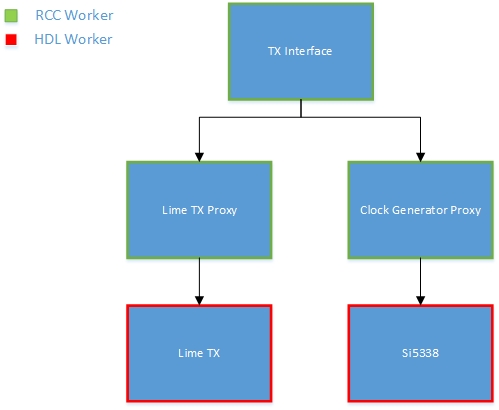
\includegraphics[scale=0.7]{matchstiq_FE_TX_toplevel}}
	\caption{Top Level Block Diagram}
	\label{fig:top}
\end{figure}
\vspace{25 mm}
\subsection*{TX Hardware}
\begin{figure}[ht]
	\centerline{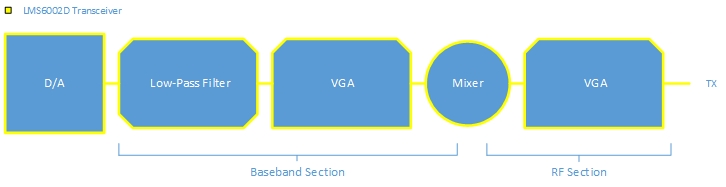
\includegraphics[scale=0.7]{matchstiq_FE_TX_HW}}
	\caption{Hardware Block Diagram}
	\label{fig:hw}
\end{figure}
\vspace{25 mm}
\newpage

\section*{Source Dependencies}
\begin{itemize}
	\item ocpi.assets/hdl/platforms/matchstiq\_z1/devices/matchstiq\_z1\_tx.rcc/matchstiq\_z1\_tx.cc
\end{itemize}

\begin{landscape}
	\section*{Component Spec Properties}
	\begin{scriptsize}
		\begin{tabular}{|p{4cm}|c|c|c|c|c|c|p{8cm}|}
			\hline
			\rowcolor{blue}
			Name                                & Type   & Sequence & Array      & Accessibility       & Valid Range & Default & Usage                                                                                                                                       \\
			\rowcolor{blue}
			                                    &        & Length   & Dimensions &                     &             &         &                                                                                                                                             \\
			\hline
			\verb+rf_gain_dB+                   & double & -        & -          & Readable, Writable  & -           & 0       & The value of the RF gain stage of the transmitter                                                                                           \\
			\hline
			\verb+rf_gain_max_dB+               & double & -        & -          & Volatile, Writable & -           & 0       & Maximum valid value for RF gain                                                                                                             \\
			\hline
			\verb+rf_gain_min_dB+               & double & -        & -          & Volatile, Writable & -           & 0       & Minimum valid value for RF gain                                                                                                             \\
			\hline
			\verb+rf_gain_step_dB+              & double & -        & -          & Volatile, Writable & -           & 0       & Minimum granularity for changes in RF gain                                                                                                  \\
			\hline
			\verb+bb_gain_dB+                   & double & -        & -          & Readable, Writable  & -           & 0       & The value of the baseband gain stage of the transmitter                                                                                     \\
			\hline
			\verb+bb_gain_max_dB+               & double & -        & -          & Volatile, Writable & -           & 0       & Maximum valid value for baseband gain                                                                                                       \\
			\hline
			\verb+bb_gain_min_dB+               & double & -        & -          & Volatile, Writable & -           & 0       & Minimum valid value for baseband gain                                                                                                       \\
			\hline
			\verb+bb_gain_step_dB+              & double & -        & -          & Volatile, Writable & -           & 0       & Minimum granularity for changes in baseband gain                                                                                            \\
			\hline
			\verb+frequency_MHz+                & double & -        & -          & Readable, Writable  & -           & 0       & The value for the tuned center frequency of the outgoing RF samples                                                                         \\
			\hline
			\verb+frequency_max_MHz+            & double & -        & -          & Volatile, Writable & -           & 0       & Maximum valid value for frequency                                                                                                           \\
			\hline
			\verb+frequency_min_MHz+            & double & -        & -          & Volatile, Writable & -           & 0       & Minimum valid value for frequency                                                                                                           \\
			\hline
			\verb+frequency_step_MHz+           & double & -        & -          & Volatile, Writable & -           & 0       & Minimum granularity for changes in frequency                                                                                                \\
			\hline
			\verb+sample_rate_MHz+              & double & -        & -          & Readable, Writable  & -           & 0       & Sample rate of the outgoing RF samples                                                                                                      \\
			\hline
			\verb+sample_rate_max_MHz+          & double & -        & -          & Volatile, Writable & -           & 0       & Maximum valid value for sample rate                                                                                                         \\
			\hline
			\verb+sample_rate_min_MHz+          & double & -        & -          & Volatile, Writable & -           & 0       & Minimum valid value for sample rate                                                                                                         \\
			\hline
			\verb+sample_rate_step_MHz+         & double & -        & -          & Volatile, Writable & -           & 0       & Minimum granularity for changes in sample rate                                                                                              \\
			\hline
			\verb+rf_cutoff_frequency_MHz+      & double & -        & -          & Readable, Writable  & -           & 0       & The cutoff frequency for any filtering that is done in the RF stage of the transmitter. Note that this property's value is equal to half of the complex bandwidth of the RF stage filter. There is no RF filtering stage on this transmitter. \\
			\hline
			\verb+rf_cutoff_frequency_max_MHz+  & double & -        & -          & Volatile, Writable & -           & 0       & Maximum valid value for RF cutoff frequency                                                                                                 \\
			\hline
			\verb+rf_cutoff_frequency_min_MHz+  & double & -        & -          & Volatile, Writable & -           & 0       & Minimum valid value for RF cutoff frequency                                                                                                 \\
			\hline
			\verb+rf_cutoff_frequency_step_MHz+ & double & -        & -          & Volatile, Writable & -           & 0       & Minimum granularity for changes in RF cutoff frequency                                                                                      \\
			\hline
			\verb+bb_cutoff_frequency_MHz+      & double & -        & -          & Readable, Writable  & -           & 0       & The cutoff frequency for any filtering that is done in the baseband stage of the transmitter. Note that this property's value is equal to half of the complex bandwidth of the baseband stage filter.                                               \\
			\hline
			\verb+bb_cutoff_frequency_max_MHz+  & double & -        & -          & Volatile, Writable & -           & 0       & Maximum valid value for baseband cutoff frequency                                                                                           \\
			\hline
			\verb+bb_cutoff_frequency_min_MHz+  & double & -        & -          & Volatile, Writable & -           & 0       & Minimum valid value for baseband cutoff frequency                                                                                           \\
			\hline
			\verb+bb_cutoff_frequency_step_MHz+ & double & -        & -          & Volatile, Writable & -           & 0       & Minimum granularity for changes in baseband cutoff frequency                                                                                \\
			\hline
		\end{tabular}
	\end{scriptsize}

	\section*{Worker Properties}
	\subsection*{\comp.rcc}
	\begin{scriptsize}
		\begin{tabular}{|p{2cm}|p{4cm}|c|c|c|c|c|c|p{6.5cm}|}
			\hline
			\rowcolor{blue}
			Type         & Name                                & Type & Sequence & Array      & Accessibility/ & Valid Range  & Default & Usage                                                                                         \\
			\rowcolor{blue}
			             &                                     &      & Length   & Dimensions & Advanced       &              &         &                                                                                               \\
			\hline
			SpecProperty & \verb+rf_gain_dB+                   & -    & -        & -          & WriteSync      & 0-25         & 4       & The value of the RF gain stage of the transmitter                                             \\
			\hline
			SpecProperty & \verb+rf_gain_max_dB+               & -    & -        & -          & -              & 25           & 25      & Maximum valid value for RF gain                                                               \\
			\hline
			SpecProperty & \verb+rf_gain_min_dB+               & -    & -        & -          & -              & 0            & 0       & Minimum valid value for RF gain                                                               \\
			\hline
			SpecProperty & \verb+rf_gain_step_dB+              & -    & -        & -          & -              & 1            & 1       & Minimum granularity for changes in RF gain                                                    \\
			\hline
			SpecProperty & \verb+bb_gain_dB+                   & -    & -        & -          & WriteSync      & -35 - -4     & -4      & The value of the baseband gain stage of the transmitter                                       \\
			\hline
			SpecProperty & \verb+bb_gain_max_dB+               & -    & -        & -          & -              & -4           & -4      & Maximum valid value for baseband gain                                                         \\
			\hline
			SpecProperty & \verb+bb_gain_min_dB+               & -    & -        & -          & -              & -35          & -35     & Minimum valid value for baseband gain                                                         \\
			\hline
			SpecProperty & \verb+bb_gain_step_dB+              & -    & -        & -          & -              & 1            & 1       & Minimum granularity for changes in baseband gain                                              \\
			\hline
			SpecProperty & \verb+frequency_MHz+                & -    & -        & -          & WriteSync      & 232.5 - 3720 & 500     & The value for the tuned center frequency of the outgoing RF samples                           \\
			\hline
			SpecProperty & \verb+frequency_max_MHz+            & -    & -        & -          & -              & 3720         & 3720    & Maximum valid value for frequency                                                             \\
			\hline
			SpecProperty & \verb+frequency_min_MHz+            & -    & -        & -          & -              & 232.5        & 232.5   & Minimum valid value for frequency                                                             \\
			\hline
			SpecProperty & \verb+frequency_step_MHz+           & -    & -        & -          & -              & 0.1          & 0.1     & Minimum granularity for changes in frequency                                                  \\
			\hline
			SpecProperty & \verb+sample_rate_MHz+              & -    & -        & -          & WriteSync      & 0.1 - 40     & 0.1     & Sample rate of the outgoing RF samples                                                        \\
			\hline
			SpecProperty & \verb+sample_rate_max_MHz+          & -    & -        & -          & -              & 40           & 40      & Maximum valid value for sample rate                                                           \\
			\hline
			SpecProperty & \verb+sample_rate_min_MHz+          & -    & -        & -          & -              & 0.1          & 0.1     & Minimum valid value for sample rate                                                           \\
			\hline
			SpecProperty & \verb+sample_rate_step_MHz+         & -    & -        & -          & -              & 1            & 1       & Minimum granularity for changes in sample rate                                                \\
			\hline
			SpecProperty & \verb+rf_cutoff_frequency_max_MHz+  & -    & -        & -          & -              & -1           & -1      & Maximum valid value for RF cutoff frequency                                                   \\
			\hline
			SpecProperty & \verb+rf_cutoff_frequency_min_MHz+  & -    & -        & -          & -              & -1           & -1      & Minimum valid value for RF cutoff frequency                                                   \\
			\hline
			SpecProperty & \verb+rf_cutoff_frequency_step_MHz+ & -    & -        & -          & -              & -1           & -1      & Minimum granularity for changes in RF cutoff frequency                                        \\
			\hline
			SpecProperty & \verb+bb_cutoff_frequency_MHz+      & -    & -        & -          & WriteSync      & 0.125-14     & 10      & The cutoff frequency for any filtering that is done in the baseband stage of the transmitter. \\
			\hline
			SpecProperty & \verb+bb_cutoff_frequency_max_MHz+  & -    & -        & -          & -              & 14           & 14      & Maximum valid value for baseband cutoff frequency                                             \\
			\hline
			SpecProperty & \verb+bb_cutoff_frequency_min_MHz+  & -    & -        & -          & -              & 0            & 0       & Minimum valid value for baseband cutoff frequency                                             \\
			\hline
			SpecProperty & \verb+bb_cutoff_frequency_step_MHz+ & -    & -        & -          & -              & 0.125        & 0.125   & Minimum granularity for changes in baseband cutoff frequency                                  \\
			\hline
		\end{tabular}
	\end{scriptsize}
\end{landscape}

\section*{Performance and Resource Utilization}
\subsubsection*{\comp.rcc}
\begin{scriptsize}
	\begin{tabular}{|c|c|c|}
		\hline
		\rowcolor{blue}
		Processor Type & Processor Frequency & Run Function Time \\
		\hline
		TBD            & TBD                 & TBD               \\
		\hline
	\end{tabular}
\end{scriptsize}

\section*{Test and Verification}
\begin{flushleft}
	The testbench for this worker is meant to exercise the properties of the worker dynamically while the application is running.  Random data is sent out to emulate noise on the spectrum analyzer.  The following steps are taken in the testbench:
	\begin{itemize}
		\item[1)] Change the rf\_gain\_dB settings
		\item[2)] Change the bb\_gain\_dB settings
		\item[3)] Toggle the low-pass filter settings
	\end{itemize}
	These steps are repeated at different center frequencies and directions are provided in the testbench for this.  The results are inspected visually on a spectrum analyzer.\par\medskip
	WARNING: A 10 dB attenuator is recommended between the radio and spectrum analyzer to prevent any equipment from being damaged.\par\medskip
	  The results should be as follows:
	\vspace{10 mm}
	\begin{figure}[ht]
		\centerline{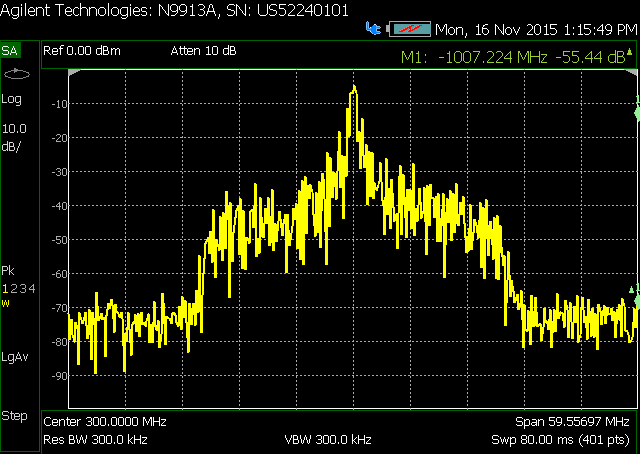
\includegraphics[scale=0.7]{NoFilter}}
		\caption{Expected Results: Beginning}
		\label{fig:tb1}
	\end{figure}
	\vspace{10 mm}
	\newpage
	\begin{figure}[ht]
		\centerline{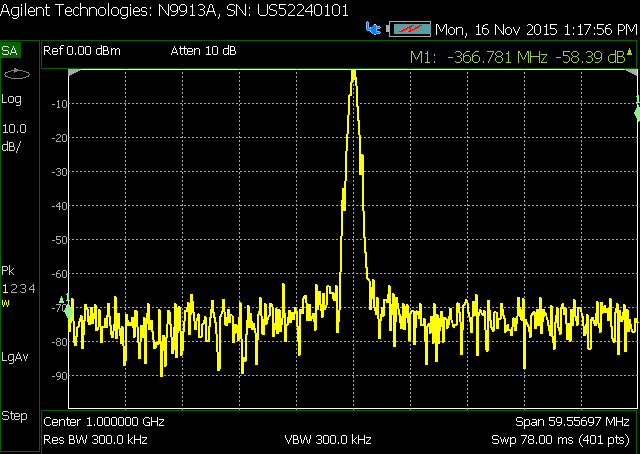
\includegraphics[scale=0.7]{YesFilter}}
		\caption{Expected Results: End}
		\label{fig:tb2}
	\end{figure}

	\vspace{15 mm}

	\noindent The signal should look like a amplitude adjusted version of the first picture throughout except when testing the filtering.  In the filtering stage of testing the signal will slowly walk from the second picture back to the first picture.
\end{flushleft}

\section*{References}
\begin{itemize}
	\item[1)] LMS6002D Datasheet, www.limemicro.com
	\item[2)] The Matchstiq-Z1 Software Development Manual (provided by Epiq with the Platform Development Kit)
\end{itemize}
\end{document}
